% document's head

\begin{center}
    \LARGE \textsc{Билеты по квантовой механике}
\end{center}

\hrule

\phantom{42}

\begin{flushright}
    \begin{tabular}{rr}
    % written by:
        % \textbf{Источник}: 
        % & \href{__ссылка__}{__название__} \\
        % & \\
        % \textbf{Лектор}: 
        % & _ФИО_ \\
        % & \\
        % \textbf{Автор заметок}: 
        \textbf{Авторы заметок}: 
        & Хоружий Кирилл \\
        & Примак Евгений \\
        & \\
    % date:
        \textbf{От}: &
        \textit{\today}\\
    \end{tabular}
\end{flushright}
\thispagestyle{empty}


\phantom{42}

\noindent
\begin{minipage}{0.5\textwidth}
     \begin{quotation}
     \noindent
        Я так давно родился, \\
        Что слышу иногда,  \\
        Как надо мной проходит \\
        Студёная вода. 

        ...

    \noindent
        Я так давно родился,  \\
        Что говорить не могу,  \\
        И город мне приснился  \\
        На каменном берегу.  \\

    \noindent
        А я лежу на дне речном  \\
        И вижу из воды  \\
        Далекий свет, высокий дом,  \\
        Зелёный луч звезды. \\
        \phantom{42} \hfill \textit{А. А. Тарковский}
    \end{quotation}
\end{minipage}


% \vfill
\phantom{42}

\phantom{42}

\phantom{42}

\hspace{20 mm} 

\phantom{42}


% \vspace*{\fill}
\begin{figure}[h]
    \centering
    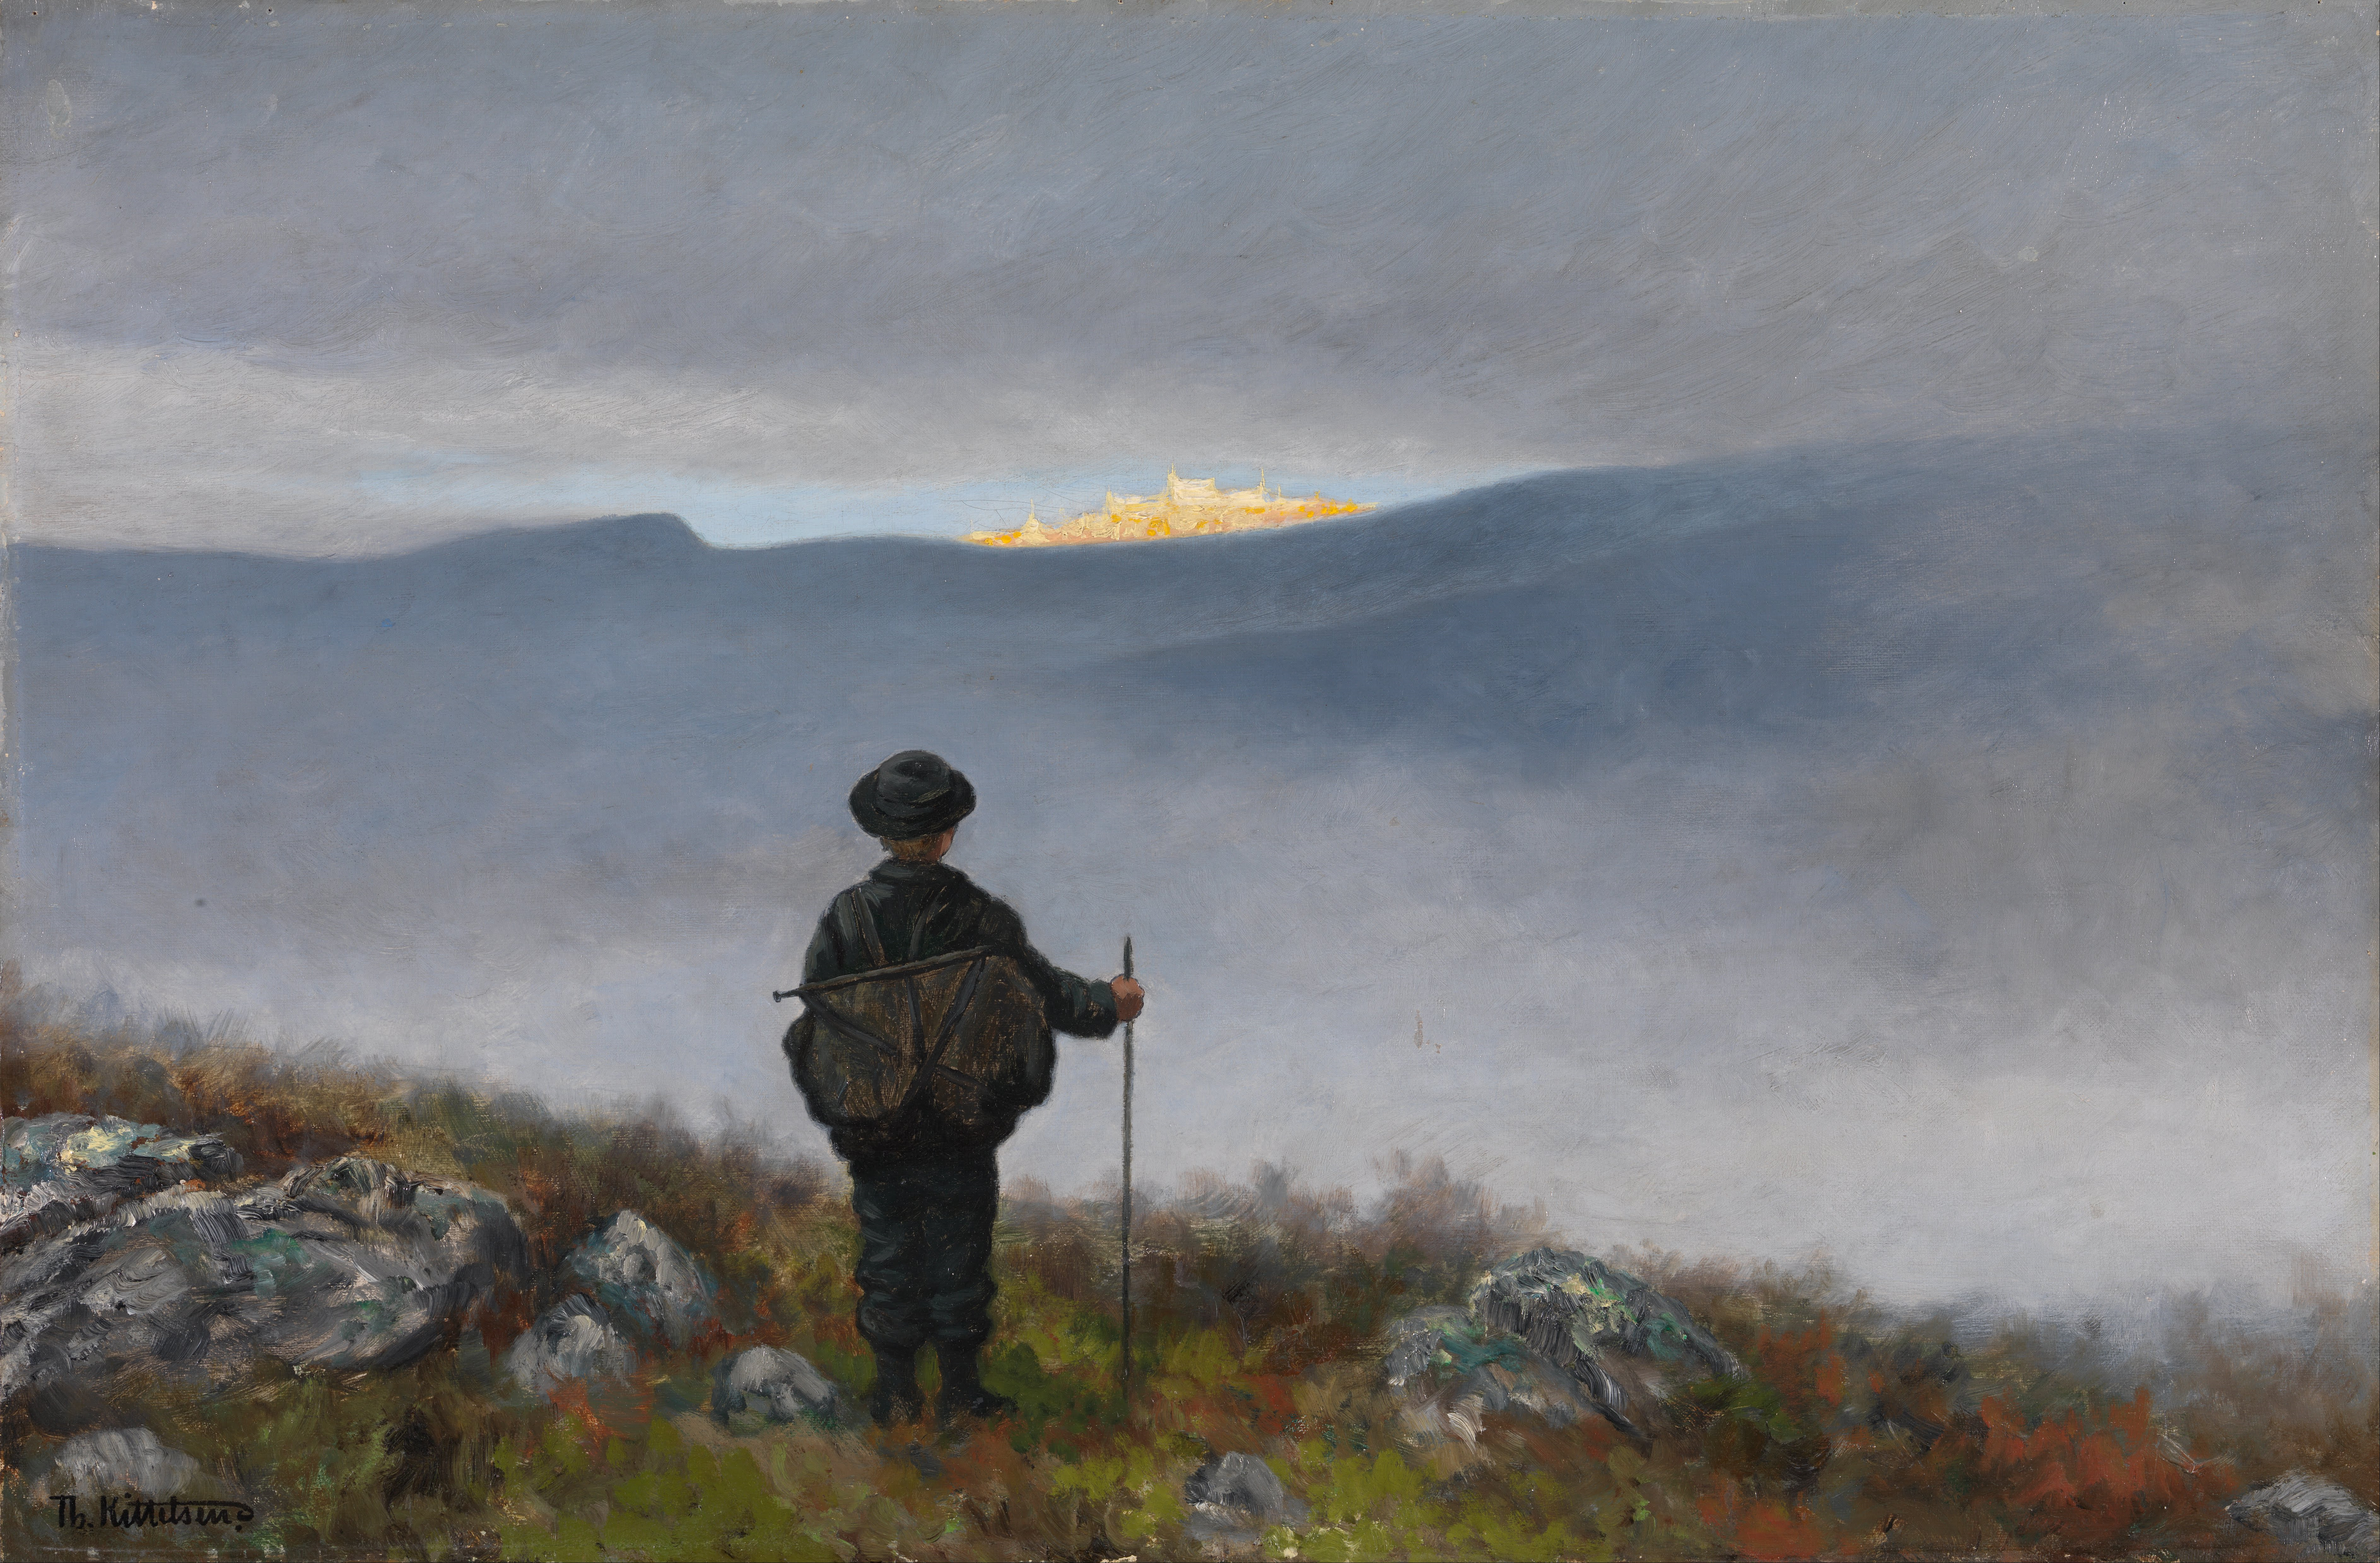
\includegraphics[width=0.95\textwidth]{figures/Kittelsen.jpg}
    %\caption{}
    %\label{fig:}
\end{figure}

% \vfill

\begin{flushright}
    \textcolor{gray}{
    \small{Также выражаем благодарность Гурьевой Соне и Мещерякову Паше за консультации по отдельным задачам.}}
\end{flushright}


\newpage

\tableofcontents
\newpage